% ============================================================
% T-DOME Paper III: The Loop
% T-DOME Program — Paper III
% ============================================================

\documentclass[12pt]{article}
\usepackage[margin=1in]{geometry}
\usepackage{amsmath,amssymb,amsthm}
\usepackage[hidelinks]{hyperref}
\usepackage{booktabs}
\usepackage{physics}
\usepackage{graphicx}
\usepackage{caption}
\usepackage{float}
\usepackage{array}
\newcolumntype{P}[1]{>{\raggedright\arraybackslash}p{#1}}
\graphicspath{{TDOME_III_supplement/}}

% Theorem environments — matching HAFF/Q-RAIF/T-DOME I/II style
\newtheorem{theorem}{Theorem}
\newtheorem{lemma}[theorem]{Lemma}
\newtheorem{proposition}[theorem]{Proposition}
\newtheorem{definition}[theorem]{Definition}
\newtheorem{remark}[theorem]{Remark}
\newtheorem{corollary}[theorem]{Corollary}
\newtheorem{conjecture}[theorem]{Conjecture}

\title{Fisher Information Geometry and Conditional Implementation Costs\\
of Self-Referential Calibration}

\author{Sidong Liu, PhD \\
\small iBioStratix Ltd \\
\small \texttt{sidongliu@hotmail.com}}

\date{July 2026}

\begin{document}
\emergencystretch=2em
\raggedbottom
\hbadness=10000
\vbadness=10000
\maketitle

% ============================================================
\begin{abstract}
Papers~I and~II of the T-DOME
series~\cite{Liu2026TDOME_I,Liu2026TDOME_II} supply conditional
resource and reference-frame models for persistent agents.  They do not
prove that all persistent agents require non-Markovian memory or
spontaneous Clifford gauge-symmetry breaking.  Paper~II's linear-drift
visibility crossover is likewise a declared coordinate model, not a
universal logarithmic ``Delusion Trap'' timescale.

This paper studies \textbf{self-referential calibration} under explicit
residual-likelihood, prior, drift, convexity, and hardware assumptions.
The agent uses the score statistics of a supplied prediction-residual
model to estimate frame mismatch.  The principal conditional results are:
\begin{enumerate}
\item \textbf{Gaussian Fisher Signal}
  (Proposition~\ref{prop:gaussian_fisher}):
  in the declared even Gaussian residual model, per-sample local Fisher
  information grows quadratically and accumulated information grows
  cubically.  Detection precedes the visibility crossover if and only if
  the threshold condition in Corollary~\ref{cor:detection_window} holds.
\item \textbf{Self-Referential Cram\'{e}r--Rao Bound}
  (Theorem~\ref{thm:SRCR}):
  the van Trees lower bound applies under the stated regular likelihood,
  conditional-independence, compact-support, and prior assumptions, with
  data and prior Fisher information entering separately.
\item \textbf{Conditional Implementation Cost}
  (Proposition~\ref{prop:loop_cost_impl}):
  a separable implementation with declared irreversible sensor and
  computational resets and linear-response actuation obeys
  $\dot{W}_{\mathrm{loop}}
  \geq k_BT\,\ln 2\,(R_s+R_c)
  + \mathcal{L}^2/\tau_{\mathrm{recalib}}^2$,
  a bound for that implementation rather than a universal cost of
  sensing, Fisher evaluation, or self-reference.
\end{enumerate}

The calibration loop has a local tracking bound only under geodesic
strong convexity and bounded drift (Theorem~\ref{thm:loop_stability}).
The four supplied layers in Definition~\ref{def:four_part_template}
define the running model architecture; they are not proved necessary,
sufficient, minimal, or complete for persistent agency.  ``Reflexivity''
here denotes one implementation of second-order control, with no claim of
architectural uniqueness or phenomenal consciousness.
\end{abstract}

% ============================================================
\section{Introduction}
\label{sec:intro}

% ------------------------------------------------------------
\subsection{Context: The Delusion Trap}
\label{subsec:delusion_context}

Revised Paper~II~\cite{Liu2026TDOME_II} studies a supplied
coordinate projection under a raw-channel budget.  It does not prove
that persistence forces Clifford gauge symmetry breaking.  Its drift
model uses a linearly changing mismatch
$\theta(t)=\theta_0+\varepsilon t$ and identifies the geometric
visibility crossover
\begin{equation}
\label{eq:t_del_recall}
t_{\mathrm{vis}}
=\frac{\pi/4-\theta_0}{\varepsilon}.
\end{equation}
That crossover does not by itself imply gradient reversal or
undetectability.  The present paper asks a narrower question: for a
specified residual likelihood, can score statistics detect mismatch,
and under what conditions can a natural-gradient controller track a
moving optimum?

% ------------------------------------------------------------
\subsection{Position within Papers~I--III}
\label{subsec:sequence}

This paper is the third and final of the T-DOME framework,
closing the three-paper sequence.

\begin{center}
\small
\setlength{\tabcolsep}{4pt}%
\begin{tabular}{@{}lP{3.5cm}P{4.2cm}c@{}}
\toprule
\textbf{Framework} & \textbf{Question} & \textbf{Result}
  & \textbf{Status} \\
\midrule
HAFF~\cite{Liu2026HAFF_A,Liu2026HAFF_B}
  & How does geometry emerge?
  & Conditional algebra/dictionary models
  & Revised \\[3pt]
Q-RAIF~\cite{Liu2026QRAIF_A,Liu2026QRAIF_B}
  & What algebra must an observer have?
  & Clifford representations as model inputs
  & Revised \\[3pt]
T-DOME~I~\cite{Liu2026TDOME_I}
  & What can inter-epoch correlations fund?
  & Restricted baseline; correlation accounting
  & Conditional \\[3pt]
T-DOME~II~\cite{Liu2026TDOME_II}
  & When can a model select a frame?
  & Conditional coordinate selection
  & Conditional \\[3pt]
\textbf{T-DOME~III} (this work)
  & How does self-calibration arise?
  & Fisher self-referential bound;
    thermodynamic cost of reflexivity
  & \textbf{This paper} \\
\bottomrule
\end{tabular}
\end{center}

The three T-DOME papers form a conditional modelling sequence:
\begin{enumerate}
\item \textbf{Paper~I:} Initial correlations can enter an ELV-type
  thermodynamic balance; a restricted autonomous baseline is proved.
\item \textbf{Paper~II:} A raw-coordinate archive motivates a supplied
  compression model and a linear visibility-crossover example.
\item \textbf{Paper~III (this work):} Uncorrected
  bias diverges from a changing environment.
  A self-referential calibration loop---monitoring the
  Fisher information of one's own prediction stream---resolves
  mismatch under explicit likelihood and convexity assumptions.  A
  conditional hardware model assigns reset and actuation costs.
\end{enumerate}

The links are motivation and model interfaces, not an irreversible
theorem chain.  None of the three papers proves that this architecture
is necessary for persistence.

% ------------------------------------------------------------
\subsection{The Information-Geometric Insight}
\label{subsec:insight}

The key observation that resolves the Delusion Trap is
subtle:
\emph{while the agent cannot observe $V_{\mathrm{bg}}$
directly, it can observe the statistical properties of its
own prediction residuals in $V_{\mathrm{fg}}$.}

The prediction residual
$e(t) := \mathcal{S}_{\mathrm{vis}}(t)
- \mathcal{S}_{\mathrm{vis}}^{(\mathrm{pred})}(t)$
lies in $V_{\mathrm{fg}}$ by construction.
In the declared even Gaussian model, a record cannot identify the sign
of mismatch.  Its \emph{distribution}---the probability law
$p(e\,|\,\sigma)$, parametrised by the gauge-fixing
parameter~$\sigma$---does depend on~$\sigma$, because the
projection $\Pi_{\mathcal{F}}(\sigma)$ determines which
environmental correlations are captured and which are
discarded.

When the frame $\sigma$ drifts away from the optimal
$\sigma^*$, the residual distribution shifts.
The \emph{Fisher information metric}
\begin{equation}
\label{eq:fisher_preview}
g_{ij}(\sigma)
= \mathbb{E}_\sigma\!\left[
  \frac{\partial \log p(e\,|\,\sigma)}
       {\partial \sigma^i}\,
  \frac{\partial \log p(e\,|\,\sigma)}
       {\partial \sigma^j}
\right]
\end{equation}
measures the sensitivity of this distribution to changes
in~$\sigma$.
Whether $g_{ij}$ changes with staleness is likelihood-dependent.  The
Gaussian model below provides one explicit case.

This is the mathematical realisation of the
``second-order operation'' demanded by
Paper~II, Section~7.5: the agent does not need to see the
truth (the full $Cl(V,q)$), but only the \emph{rate of
change of its own prediction error} as a function of its
frame parameters.
Fisher information is one local sensitivity measure, not the unique
possible detector.

% ------------------------------------------------------------
\subsection{Relation to Architectural Incompleteness}
\label{subsec:haff_g}

Revised HAFF Paper~G~\cite{Liu2026HAFF_G} supplies
philosophy-of-science motivation rather than a fixed-point no-go
theorem.  In that motivational sense,
the self-referential calibration loop cannot \emph{eliminate}
architectural incompleteness, but it can \emph{track}
the consequences of incompleteness in real time.
The Lyapunov function $V(\sigma)$ monitors the distance
between the agent's frame and the optimal frame without
requiring access to the ``complete'' description---it
operates entirely within the agent's own predictive
statistics.

% ------------------------------------------------------------
\subsection{Scope and Disclaimers}
\label{subsec:scope}

\begin{enumerate}
\item \emph{Reflexivity} refers throughout to
  second-order control: the ability of a system to
  monitor and adjust its own monitoring process.
  It carries \emph{no} implication of phenomenal
  consciousness, subjective experience, or qualia.
\item The self-referential calibration loop does not
  \emph{eliminate} the ego's bias; it tracks and
  compensates for drift in the bias.
  The four bias terms of Paper~II persist in the
  calibrated phase.
\item The thermodynamic cost statement is conditional on irreversible
  reset, separable hardware, and a linear-response actuation model.
\item The framework applies to systems
  satisfying~(C1)--(C5) (Section~\ref{subsec:standing_C}).
  It is not a universal theory of agency.
\end{enumerate}

\paragraph{Related work.}
The Fisher information metric on statistical manifolds was
introduced by Rao~\cite{Rao1945} and shown to be unique
by \v{C}encov~\cite{Cencov1982}.
The natural gradient and information geometry were developed
by Amari~\cite{Amari1998,AmariNagaoka2000}.
Thermodynamic length and optimal finite-time transformations
were established by
Crooks~\cite{Crooks2007} and
Sivak--Crooks~\cite{SivakCrooks2012}.
The connection between Fisher information and entropy
production was formalised by Ito~\cite{Ito2018} and
Barato--Seifert~\cite{BaratoSeifert2015}.
Second-order cybernetics originates with
Ashby~\cite{Ashby1956} and
von Foerster~\cite{vonFoerster2003}.
Adaptive control and self-tuning regulators are treated
in~\cite{AstromWittenmark1995}.
The Bayesian Cram\'{e}r--Rao bound (van Trees inequality)
is from~\cite{vanTrees1968}.

\paragraph{Summary of contributions.}
This paper separates three levels of result:
\begin{enumerate}
\item \textbf{Drift Detectability}
  (Proposition~\ref{prop:gaussian_fisher}): an explicit Gaussian
  residual likelihood has quadratic per-sample and cubic accumulated
  local Fisher signals; early detection is a threshold condition.
\item \textbf{Self-Referential Cram\'{e}r--Rao Bound}
  (Theorem~\ref{thm:SRCR}):
  drift-estimation precision is bounded by the sum of
  data Fisher information and ego rigidity.
\item \textbf{Thermodynamic Cost}
  (Proposition~\ref{prop:loop_cost_impl}): a separable implementation
  with irreversible resets and finite-time actuation obeys a conditional
  additive bound.
\end{enumerate}

\paragraph{Result-status ledger.}
The original drift-detectability theorem
\texttt{TD-III-T3.3} is retracted;
Proposition~\ref{prop:gaussian_fisher} is an FD/I model calculation and
Corollary~\ref{cor:detection_window} is conditional on a declared
threshold.  Ego rigidity \texttt{TD-III-ego} remains a supplied prior
model.  The tracking theorem is conditional on local geodesic strong
convexity.  The universal additive-cost claim
\texttt{TD-III-T6.2} is downgraded to
Proposition~\ref{prop:loop_cost_impl}, and the inherited persistence
budget is withdrawn.

% ============================================================
\section{Mathematical Preliminaries}
\label{sec:prelim}

% ------------------------------------------------------------
\subsection{Inherited Framework from Papers~I and~II}
\label{subsec:inherited}

We briefly recall the key objects; the reader is referred to
Papers~I and~II for full definitions and proofs.

\paragraph{From Paper~I~\cite{Liu2026TDOME_I}.}
\begin{itemize}
\item \textbf{Survival functional.}
  $\mathcal{S}[\Lambda,\tau]
  := \Delta F - W[0,\tau]$~(Paper~I,
  Eq.~(9)).
\item \textbf{Restricted autonomous baseline.}
  $\mathcal{S}[\Lambda^{\mathrm{D}},\tau]\leq0$ for a fixed-Hamiltonian,
  no-control Davies semigroup under its stated initial conditions.  It
  is not a ceiling for all Markovian agents.
\item \textbf{Memory kernel.}
  $\mathcal{K}(t,s)$: the non-Markovian superoperator
  encoding system--environment correlations.
\item \textbf{Entropy rate.}
  $h_\mu := \lim_{T\to\infty}T^{-1}H(X_{0:T})$ (bits per
  unit time per algebraic component).
\item \textbf{Predictive information.}
  $I_{\mathrm{pred}}
  := I(\overleftarrow{X};\,\overrightarrow{X})$.
\end{itemize}

\paragraph{From Paper~II~\cite{Liu2026TDOME_II}.}
\begin{itemize}
\item \textbf{Internal algebra.}
  $\mathcal{O}_{\mathrm{int}} = Cl(V,q)$, $D = \dim Cl(V,q) = 2^n$,
  gauge group $G = \mathrm{Aut}(Cl(V,q))$.
\item \textbf{Gauge bundle.}
  $\pi: P \to M$, structure group $G$; a section
  $\sigma: M \to P$ is a reference frame.
\item \textbf{Ego.}
  $\mathfrak{E} := (\mathcal{F}^*,\,V_{\mathrm{fg}}^*)$
  denotes a chosen optimizer in a supplied encoder class, with
  $k^*=k_{\mathrm{opt}}\leq k_{\max}$.  The budget capacity is not a
  universal optimizer formula.
\item \textbf{Projected kernel.}
  $\mathcal{K}_{\mathcal{F}}(t,s)
  = \Pi_{\mathcal{F}}\,\mathcal{K}(t,s)\,
  \Pi_{\mathcal{F}}$.
\item \textbf{Survival decomposition.}
  $\mathcal{S} = \mathcal{S}_{\mathrm{vis}}(\mathcal{F})
  + \mathcal{S}_{\mathrm{hid}}(\mathcal{F})$.
\item \textbf{Four bias terms.}
  $\mathcal{B}_{\mathrm{select}}$,
  $\mathcal{B}_{\mathrm{frame}}$,
  $\mathcal{B}_{\mathrm{center}}$,
  $\mathcal{B}_{\mathrm{inc}}$
  (revised Paper~II, four-diagnostics definition).  These are model
  diagnostics, not generic consequences of gauge fixing.
\item \textbf{Visibility crossover.}
  $t_{\mathrm{vis}}=(\pi/4-\theta_0)/\varepsilon$ in the supplied
  linear drift geometry.  Gradient reversal requires an additional
  controller condition.
\item \textbf{Information objects.}
  Mutual information is evaluated on explicitly induced record
  processes; algebra symbols are not themselves random variables.
\end{itemize}

% ------------------------------------------------------------
\subsection{Fisher Information Metric}
\label{subsec:fisher}

\begin{definition}[Fisher information matrix]
\label{def:fisher}
Let $\{p(x\,|\,\theta) : \theta \in \Theta
\subset \mathbb{R}^d\}$ be a parametric family of
probability densities satisfying standard regularity
conditions (interchange of differentiation and integration).
The \emph{Fisher information matrix} is
\begin{equation}
\label{eq:fisher_def}
g_{ij}(\theta)
:= \mathbb{E}_\theta\!\left[
  \frac{\partial \log p(x\,|\,\theta)}
       {\partial \theta^i}\,
  \frac{\partial \log p(x\,|\,\theta)}
       {\partial \theta^j}
\right]
= -\mathbb{E}_\theta\!\left[
  \frac{\partial^2 \log p(x\,|\,\theta)}
       {\partial \theta^i\,\partial \theta^j}
\right].
\end{equation}
The pair $(\Theta,\,g)$ is a Riemannian manifold called the
\emph{statistical manifold}.
\end{definition}

\begin{remark}[Uniqueness]
\label{rem:cencov}
By \v{C}encov's theorem~\cite{Cencov1982}, the Fisher--Rao
metric $g^{\mathrm{FR}}$ is, up to a positive scalar
multiple, the unique Riemannian metric on the space of
probability distributions that is invariant under all
Markov morphisms (sufficient-statistic embeddings).
Within the hypotheses and category used by \v{C}encov's theorem, this
makes the Fisher metric a canonical local distinguishability metric.
It does not make a Fisher-based detector physically mandatory, nor does
it choose a likelihood or control objective for the agent.
\end{remark}

\begin{proposition}[Cram\'{e}r--Rao bound]
\label{prop:CR}
For any unbiased estimator $\hat{\theta}$ of $\theta$ based
on $n$ independent observations:
\begin{equation}
\label{eq:CR}
\mathrm{Cov}(\hat{\theta})
\;\succeq\; \frac{1}{n}\,\bigl[g(\theta)\bigr]^{-1}
\end{equation}
in the L\"{o}wner order.
The scalar case reads
$\mathrm{Var}(\hat{\theta})
\geq 1/\bigl(n\,g(\theta)\bigr)$.
\end{proposition}

\begin{remark}[Effective independence]
\label{rem:effective_independence}
Throughout this paper, references to ``independent
observations'' in the context of continuous-time residual
streams should be read as \emph{effective independence}
after thinning by the environmental decorrelation
time~$\tau_E$, yielding an effective sample size
$n_{\mathrm{eff}} \approx T/\tau_E$.
In particular, the sample count $n$ in~\eqref{eq:CR}
becomes $n_{\mathrm{eff}}$ in the self-referential
setting of Section~\ref{subsec:SRCR}.
\end{remark}

\begin{remark}[Fisher metric and KL divergence]
\label{rem:fisher_KL}
The Fisher metric arises as the Hessian of the
Kullback--Leibler divergence~\cite{CoverThomas2006}:
\begin{equation}
\label{eq:fisher_KL}
D_{\mathrm{KL}}\bigl(p_\theta \,\|\, p_{\theta+d\theta}\bigr)
= \tfrac{1}{2}\,g_{ij}(\theta)\,d\theta^i\,d\theta^j
  + O\!\left(|d\theta|^3\right).
\end{equation}
This identifies the Fisher metric as the infinitesimal
measure of statistical distinguishability.
\end{remark}

% ------------------------------------------------------------
\subsection{Information Geometry}
\label{subsec:info_geom}

Following Amari~\cite{Amari1985,AmariNagaoka2000}, the
statistical manifold $(\Theta,\,g)$ carries additional
geometric structure beyond the Riemannian metric.

\paragraph{$\alpha$-connections.}
For each $\alpha \in [-1,\,1]$, Amari defines an affine
connection $\nabla^{(\alpha)}$ on $\Theta$.
The cases $\alpha = 1$ (exponential connection,
$\nabla^{(e)}$) and $\alpha = -1$ (mixture connection,
$\nabla^{(m)}$) are \emph{dual} with respect to $g$:
$\partial_k\,g(X,Y)
= g(\nabla_k^{(e)}X,\,Y)
+ g(X,\,\nabla_k^{(m)}Y)$.
For exponential families, $\nabla^{(e)}$ is flat in natural
parameters and $\nabla^{(m)}$ is flat in expectation
parameters---the \emph{dually flat structure}.
The case $\alpha = 0$ recovers the Levi-Civita connection of
the Fisher metric.

\paragraph{Natural gradient.}
Standard gradient descent in parameter space ignores the
curvature of the statistical manifold.
The \emph{natural gradient}~\cite{Amari1998}
\begin{equation}
\label{eq:natural_gradient}
\dot{\theta}
= -\eta\,g^{-1}(\theta)\,\nabla_\theta L(\theta),
\end{equation}
where $\eta > 0$ is the learning rate and $L(\theta)$ is a
loss function, provides the steepest descent direction in the
Fisher metric.
It is reparametrisation-invariant.  Statistical efficiency requires
additional estimator and asymptotic assumptions and is not implied by
the update formula alone.

\paragraph{Pythagorean theorem.}
In a dually flat space, the KL divergence satisfies
a generalised Pythagorean relation:
$D_{\mathrm{KL}}(p\,\|\,r)
= D_{\mathrm{KL}}(p\,\|\,q)
+ D_{\mathrm{KL}}(q\,\|\,r)$
when $q$ is the $m$-projection of $p$ onto a
submanifold containing $r$.
This decomposition will be applied to separate the
foreground-recoverable and background-irrecoverable
components of drift.

% ------------------------------------------------------------
\subsection{Thermodynamic Length}
\label{subsec:thermo_length}

\begin{definition}[Thermodynamic length]
\label{def:thermo_length}
Let $\lambda(t)$ for $t \in [0,\tau]$ be a path through
control parameter space, and let $\zeta_{ij}(\lambda)$ be the
\emph{friction tensor} (the time-integrated equilibrium
force--force correlation function at~$\lambda$).
The \emph{thermodynamic length} of the
path~\cite{Crooks2007} is
\begin{equation}
\label{eq:thermo_length}
\mathcal{L}
:= \int_0^\tau
\sqrt{\zeta_{ij}(\lambda)\,
  \dot{\lambda}^i\,\dot{\lambda}^j}\;dt.
\end{equation}
\end{definition}

\begin{proposition}[Sivak--Crooks bound]
\label{prop:sivak_crooks}
The excess (dissipated) work during a finite-time
transformation of duration $\tau$ satisfies~\cite{SivakCrooks2012}
\begin{equation}
\label{eq:sivak_crooks}
W_{\mathrm{ex}} \;\geq\; \frac{\mathcal{L}^2}{\tau}.
\end{equation}
The minimum is achieved by the geodesic of the friction
tensor $\zeta$.
In the linear-response regime, the friction tensor is
related to the Fisher metric of the equilibrium distribution
at $\lambda$ by
$\zeta_{ij}(\lambda)
\sim \tau_{\mathrm{relax}}\,g_{ij}^{\mathrm{Fisher}}(\lambda)$,
where $\tau_{\mathrm{relax}}$ is the relaxation time.
\end{proposition}

% ------------------------------------------------------------
\subsection{Second-Order Cybernetics}
\label{subsec:cybernetics}

Von Foerster~\cite{vonFoerster2003} distinguished two levels
of control:
\begin{itemize}
\item \textbf{First-order cybernetics}: feedback control of
  observed systems.
  The controller adjusts its actions based on the output of
  a sensor.
  Paper~II's ego is a first-order structure: it processes
  environmental data within a fixed frame.
\item \textbf{Second-order cybernetics}: feedback control of
  the \emph{observing} system itself.
  The controller adjusts the \emph{sensor}---or equivalently,
  the reference frame within which the sensor operates.
  This is what Paper~III provides.
\end{itemize}

Ashby's Law of Requisite Variety~\cite{Ashby1956} provides a
lower bound on the complexity of the meta-controller:
\begin{equation}
\label{eq:requisite_variety}
\dim\!\left(\text{meta-controller state space}\right)
\;\geq\; \dim\!\left(\text{environmental drift subspace}\right).
\end{equation}
The meta-observer must have at least as many adjustable
parameters as there are independent modes of environmental
drift.

In adaptive control
theory~\cite{AstromWittenmark1995}, the analogous result is
the \emph{persistent excitation} condition: parameter
estimates converge if and only if the input signal is
``rich enough'' to excite all modes of the system.
In our framework, persistent excitation corresponds to
$h_\mu > 0$---the environment must continue to generate
novelty for the self-calibration loop to function.

\begin{remark}[Operational content]
\label{rem:cybernetics_operational}
The second-order cybernetic structure in this paper is
\emph{not} a philosophical metaphor.
It has concrete operational content: the natural gradient
update~\eqref{eq:natural_gradient} is a specific algorithm
that takes as input the Fisher information of the residual
stream and produces as output an update to the frame
parameter~$\sigma$.
An implementation must supply a differentiable residual likelihood,
evaluate or approximate its score, and realize the update law.  Merely
accumulating an unlabelled residual second moment is not generally a
Fisher computation.
\end{remark}

% ------------------------------------------------------------
\subsection{Standing Assumptions}
\label{subsec:standing_C}

\begin{definition}[Standing Assumptions]
\label{def:assumptions_C}
Throughout this paper, the following conditions are assumed:
\begin{enumerate}
\item[\textup{(C1)}] \textbf{Supplied representation model.}
  A finite-dimensional agent model, a foreground projection, and a
  control algebra are specified.  A Clifford representation and any
  external map $\phi$ are model inputs, not conclusions inherited from
  revised Q-RAIF or T-DOME II.
\item[\textup{(C2)}] \textbf{Environmental drift.}
  The instantaneous optimal frame
  $\mathcal{F}^*(t)$ rotates continuously in~$G$ at
  bounded speed.  In the scalar worked model the mismatch is
  $\theta(t)=\theta_0+\varepsilon t$ up to the first visibility
  crossover, as in revised Paper~II.
\item[\textup{(C3)}] \textbf{Finite meta-observer budget.}
  The self-calibration loop has a computational budget
  $\mathcal{C}_{\mathrm{meta}} < \infty$ (bits per unit
  time), distinct from the ego's processing budget
  $\mathcal{C}_{\mathrm{budget}}$.
\item[\textup{(C4)}] \textbf{Regularity.}
  The agent's predictive family
  $\{p(e\,|\,\sigma)
  : \sigma \in G/H\}$ satisfies standard Fisher
  information regularity: finite Fisher matrix and interchange of
  differentiation and integration.  Any scalar sensitivity or uniform
  lower bound used later must be assumed separately.
\item[\textup{(C5)}] \textbf{Persistent excitation.}
  The time-averaged Fisher matrix obeys the explicit lower bound in
  Definition~\ref{def:PE_constant}.  A positive entropy rate alone is
  not sufficient for this condition.
\end{enumerate}
\end{definition}

% ============================================================
\section{The Drift Detection Problem}
\label{sec:detection}

% ------------------------------------------------------------
\subsection{Identifiability in an Even Residual Model}
\label{subsec:first_order}

\begin{proposition}[Sign non-identifiability in an even residual model]
\label{prop:first_order_nonidentifiability}
Suppose the scalar residual model is
$e\mid\theta\sim\mathcal N(a\theta^2,\sigma_e^2)$ with
$a\neq0$ and $\sigma_e>0$.  Then
$p(e\mid\theta)=p(e\mid-\theta)$ for every sample and every
record length.  Residual data alone therefore cannot identify the sign
of the frame mismatch without an orientation-breaking input.
\end{proposition}

\begin{proof}
The likelihood depends on $\theta$ only through $\theta^2$; hence the
joint likelihood of any record is invariant under
$\theta\mapsto-\theta$.  No statistic of that record can distinguish
the two parameter values.
\end{proof}

This proposition is a property of the declared even likelihood.  It
does not prove that every instantaneous or ``first-order'' controller
fails: directional probes, asymmetric residual models, and exogenous
orientation data can remove the ambiguity.

% ------------------------------------------------------------
\subsection{The Agent's Statistical Manifold}
\label{subsec:stat_manifold}

The agent's prediction-residual stream
$\{e(t)\}_{t \geq 0}$ defines a stochastic process whose
distribution depends on the gauge-fixing
parameter~$\sigma$.
We model this dependence as a parametric family.

\begin{definition}[Predictive family]
\label{def:predictive_family}
The \emph{predictive family} of the agent is the set
\begin{equation}
\label{eq:predictive_family}
\mathcal{P}
:= \bigl\{p(e\,|\,\sigma)
  : \sigma \in \mathcal{M}_G\bigr\},
\end{equation}
where $\mathcal{M}_G := G/H$ is the space of gauge-fixing
orbits ($H$ is the stabiliser of the foreground subspace),
$e$ denotes the prediction-residual time series over a
window of length~$T$, and $p(e\,|\,\sigma)$ is the
likelihood of the observed residuals given the gauge
parameter~$\sigma$.
\end{definition}

The key insight is that $p(e\,|\,\sigma)$ depends
on~$\sigma$ even though $e(t) \in V_{\mathrm{fg}}$,
because the projection $\Pi_{\mathcal{F}}(\sigma)$
determines which environmental correlations are captured.
When $\sigma$ drifts from the optimal $\sigma^*$:
\begin{itemize}
\item The variance of the residuals increases (the
  discarded background components contribute unmodelled
  noise).
\item The temporal correlations of the residuals change
  (the projected kernel $\mathcal{K}_{\mathcal{F}}$ no
  longer captures the dominant environmental modes).
\item Higher-order statistics (kurtosis, spectral shape)
  shift systematically.
\end{itemize}
These distributional changes are invisible to the
raw error $e(t)$ but detectable by the Fisher metric
of $\mathcal{P}$.

% ------------------------------------------------------------
\subsection{Self-Referential Fisher Information}
\label{subsec:self_ref_fisher}

\begin{definition}[Self-referential Fisher information]
\label{def:self_ref_fisher}
For one residual with likelihood $p(e\mid\sigma)$, define the
\emph{per-sample Fisher information}
\begin{equation}
\label{eq:self_ref_fisher}
\mathcal I_1(\sigma)
:=\mathbb E_\sigma\!\left[
  (\partial_\sigma\log p(e\mid\sigma))^2\right].
\end{equation}
For conditionally independent residuals observed at times $t_m$, the
\emph{accumulated local information} is
$J_T:=\sum_{t_m\leq T}\mathcal I_1(\sigma(t_m))$.
The Fisher metric $g$, the local quadratic form
$g_{ij}\delta\sigma^i\delta\sigma^j$, and $J_T$ are distinct
objects.  Fisher information is measured in inverse-squared parameter
units, not bits.
\end{definition}

\begin{remark}[What the agent ``measures'']
\label{rem:what_measured}
Computing $\mathcal I_1(\sigma)$ does not require access
to $V_{\mathrm{bg}}$ or to the ``true'' environment.
It requires only: (i)~the agent's own prediction residuals
$\{e(t)\}$ (which lie in $V_{\mathrm{fg}}$), and
(ii)~the ability to evaluate the score function
$\partial_\sigma \log p(e\,|\,\sigma)$---the sensitivity of
its own predictive model to frame perturbations.
This is a computation entirely within the agent's internal
algebra, using only quantities already available from the
ego's processing pipeline.
\end{remark}

\begin{proposition}[Fisher signal in a Gaussian residual model]
\label{prop:gaussian_fisher}
Let residuals sampled at rate $r$ be conditionally independent with
\begin{equation}
\label{eq:gaussian_residual}
e_m\mid\theta_m\sim\mathcal N(a\theta_m^2,\sigma_e^2),
\qquad \theta(t)=\theta_0+\varepsilon t,
\end{equation}
where $a\neq0$, $\sigma_e>0$, and $\varepsilon>0$.  The per-sample
Fisher information with respect to the current mismatch is
\begin{equation}
\label{eq:detectability}
\mathcal I_1(\theta)=\frac{4a^2\theta^2}{\sigma_e^2}.
\end{equation}
Consequently the expected accumulated local information over a window
of length $T$ is
\begin{equation}
\label{eq:accumulated_fisher}
J_T\simeq\frac{4a^2r}{3\sigma_e^2\varepsilon}
\left[(\theta_0+\varepsilon T)^3-\theta_0^3\right].
\end{equation}
For a freshly calibrated frame ($\theta_0=0$), the per-sample signal is
quadratic in time and $J_T=4a^2r\varepsilon^2T^3/(3\sigma_e^2)$.
\end{proposition}

\begin{proof}
For a normal family with fixed variance and mean
$\mu(\theta)=a\theta^2$, the score is
$(e-\mu)\mu'(\theta)/\sigma_e^2$.  Taking its squared
expectation gives $(\mu')^2/\sigma_e^2$, which is
\eqref{eq:detectability}.  Summing over samples and using the sampling
rate gives
$J_T\simeq r\int_0^T\mathcal I_1(\theta_0+\varepsilon t)dt$,
which evaluates to~\eqref{eq:accumulated_fisher}.
\end{proof}

\begin{remark}[Scope of the sensitivity claim]
\label{rem:fisher_sensitivity_scope}
Full-rank Fisher information for $\sigma$ does not imply that a scalar
mismatch map $\theta(\sigma)$ has a Jacobian bounded away from zero.
Proposition~\ref{prop:gaussian_fisher} therefore works directly in the
identified scalar mismatch coordinate.  A multi-parameter extension
must supply or derive the relevant sensitivity map.
\end{remark}

\begin{corollary}[Conditional detection before visibility crossover]
\label{cor:detection_window}
In the Gaussian residual model, let $J_{\min}>0$ be a declared
detection threshold.  For a freshly calibrated frame,
\begin{equation}
\label{eq:detection_window}
T_{\mathrm{det}}
=\left(\frac{3\sigma_e^2J_{\min}}
  {4a^2r\varepsilon^2}\right)^{1/3}.
\end{equation}
Detection precedes Paper~II's visibility crossover if and only if
$T_{\mathrm{det}}<t_{\mathrm{vis}}$, where for the same linear drift
$t_{\mathrm{vis}}=(\pi/4-\theta_0)/\varepsilon$.  Equivalently, for
general $\theta_0$ the condition is
$J_{t_{\mathrm{vis}}}>J_{\min}$.  No unconditional ordering follows
from regularity alone.
\end{corollary}

\begin{proof}
Set the fresh-calibration expression for $J_T$ in
Proposition~\ref{prop:gaussian_fisher} equal to $J_{\min}$ and solve
for $T$.  Comparing that value with the independently defined
visibility time gives the stated condition.
\end{proof}

% ============================================================
\section{The Self-Referential Bound}
\label{sec:SRCR}

% ------------------------------------------------------------
\subsection{The Bayesian Framework}
\label{subsec:bayesian}

The agent's ego structure (Paper~II) provides a
\emph{prior belief} about the correct gauge parameter:
the current frame $\sigma_0$ is the ego's
``preferred'' value.
We encode this as a prior distribution
$\pi_{\mathrm{ego}}(\sigma)$, concentrated around
$\sigma_0$.

\begin{definition}[Ego rigidity]
\label{def:ego_rigidity}
The \emph{ego rigidity} is the prior Fisher information
\begin{equation}
\label{eq:ego_rigidity}
\mathcal{I}_{\mathrm{ego}}
:= \int_{\mathcal{M}_G}
\left(\frac{\partial \log \pi_{\mathrm{ego}}(\sigma)}
  {\partial \sigma}\right)^{\!2}
\pi_{\mathrm{ego}}(\sigma)\,d\sigma.
\end{equation}
High $\mathcal{I}_{\mathrm{ego}}$ corresponds to a
sharply peaked prior (rigid ego); low
$\mathcal{I}_{\mathrm{ego}}$ to a diffuse prior (flexible
ego).
This prior and its Fisher information are supplied model data.  The
diagnostics of Paper~II do not determine a prior without an additional
statistical construction.
\end{definition}

% ------------------------------------------------------------
\subsection{The Self-Referential Cram\'{e}r--Rao Bound}
\label{subsec:SRCR}

\begin{theorem}[Self-Referential Cram\'{e}r--Rao Bound]
\label{thm:SRCR}
Let the scalar drift parameter $\delta\sigma$ lie in a compact interval
$[a,b]$.  Assume that the residual likelihood is regular, that the
effective samples are conditionally independent, and that the prior
$\pi_{\mathrm{ego}}$ is $C^1$, has finite prior Fisher information,
and vanishes at $a$ and $b$.  Let $\delta\hat\sigma$ be any estimator
based only on a residual record of duration~$T$.
Define the \emph{effective sample size}
$n_{\mathrm{eff}} := T/\tau_E$, where $\tau_E$ is the
decorrelation time of the residual process~$\{e(t)\}$
(the time beyond which consecutive residuals carry
approximately independent information about~$\sigma$).
If the effective samples share per-sample information
$\mathcal I_1(\delta\sigma)$, the van Trees
inequality~\cite{vanTrees1968} gives
\begin{equation}
\label{eq:SRCR}
\mathbb{E}\!\left[
  \bigl|\delta\hat{\sigma} - \delta\sigma\bigr|^2
\right]
\;\geq\; \frac{1}{
  n_{\mathrm{eff}}\,\mathbb E_{\pi}[\mathcal I_1(\delta\sigma)]
  + \mathcal{I}_{\mathrm{ego}}}.
\end{equation}
\end{theorem}

\begin{proof}
This is a direct application of the van Trees
(Bayesian Cram\'{e}r--Rao)
inequality~\cite{vanTrees1968}.
The total information about the drift parameter $\delta\sigma$
consists of two contributions:
\begin{itemize}
\item $n_{\mathrm{eff}}\,\mathbb E_\pi[\mathcal I_1]$: the data
  Fisher information.  In continuous time, the residual
  process is correlated with decorrelation time $\tau_E$
  set by the bath memory kernel.
  Over a window of duration~$T$, the process yields
  $n_{\mathrm{eff}} \approx T/\tau_E$ effectively
  independent samples, each carrying Fisher information
  about $\delta\sigma$.
\item $\mathcal{I}_{\mathrm{ego}}$: the prior Fisher
  information from the ego's preference for $\sigma_0$
  (Definition~\ref{def:ego_rigidity}).
\end{itemize}
The boundary and regularity assumptions remove the
integration-by-parts boundary term in the standard van Trees proof.
Fisher information is not measured in bits; the denominator has
inverse-squared parameter units.
\end{proof}

\begin{remark}[The ego as help and hindrance]
\label{rem:ego_dual}
The ego rigidity $\mathcal{I}_{\mathrm{ego}}$ acts as
both help and hindrance:
\begin{itemize}
\item \textbf{Help}: when the ego is well-aligned
  ($\sigma_0 \approx \sigma^*$), the prior tightens the
  bound, reducing estimation variance.
\item \textbf{Hindrance}: when the ego is misaligned
  ($|\sigma_0 - \sigma^*|$ large), the prior pulls the
  estimate toward the wrong value, creating a
  \emph{confirmation bias} that resists recalibration.
\end{itemize}
For a conjugate scalar Gaussian location model only, the posterior mean
has the precision-weighted form below, where
$\bar{\mathcal I}_1$ is its constant per-sample data precision:
\begin{equation}
\label{eq:optimal_estimator}
\hat{\sigma}_{\mathrm{opt}}
= \frac{n_{\mathrm{eff}}\,\bar{\mathcal I}_1\,\hat{\sigma}_{\mathrm{MLE}}
  + \mathcal{I}_{\mathrm{ego}}\,\sigma_0}
  {n_{\mathrm{eff}}\,\bar{\mathcal I}_1 + \mathcal{I}_{\mathrm{ego}}},
\end{equation}
a weighted average of the maximum-likelihood estimate
$\hat{\sigma}_{\mathrm{MLE}}$ and the ego's prior belief
$\sigma_0$, with weights proportional to their respective
Fisher informations.
This formula is not implied by van Trees for a general likelihood or
prior.  In the conjugate Gaussian case, as
$n_{\mathrm{eff}}\,\bar{\mathcal I}_1 \gg \mathcal{I}_{\mathrm{ego}}$
(enough data to overwhelm the ego), the estimator converges
to the MLE.
\end{remark}

% ------------------------------------------------------------
\subsection{The Rigidity-Sensitivity Trade-off}
\label{subsec:rigidity}

\begin{proposition}[Optimal ego rigidity]
\label{prop:optimal_rigidity}
Let the total expected loss be
$\mathcal{L}_{\mathrm{total}}
(\mathcal{I}_{\mathrm{ego}})
= \mathcal{L}_{\mathrm{estimation}}
+ \lambda\,\mathcal{L}_{\mathrm{calibration}}$,
where $\mathcal{L}_{\mathrm{estimation}}$ is the
mean-squared drift-estimation error
(bounded by~\eqref{eq:SRCR}) and
$\mathcal{L}_{\mathrm{calibration}}$ is the cost of
adjusting the frame (proportional to the frame rotation
distance, hence larger when the ego is rigid and must be
overcome).
If the admissible rigidity interval is nonempty and compact and the two
supplied loss terms are lower semicontinuous, an optimal rigidity
$\mathcal{I}_{\mathrm{ego}}^*$ exists.  Uniqueness or an interior
optimum additionally requires a model-specific strict-convexity or
monotonicity condition.

\emph{Too rigid}
($\mathcal{I}_{\mathrm{ego}} \gg n_{\mathrm{eff}}\,\bar{\mathcal I}_1$):
the ego overwhelms the data; the agent is blind to drift.
\emph{Too soft}
($\mathcal{I}_{\mathrm{ego}} \ll n_{\mathrm{eff}}\,\bar{\mathcal I}_1$):
the agent overreacts to noise; calibration cost is high.
The optimum balances sensitivity against stability.
\end{proposition}

\begin{proof}
A lower-semicontinuous real function attains its minimum on a nonempty
compact set.  The existence conclusion uses only that fact; the
qualitative ``too rigid/too soft'' interpretation is not a convexity
proof.
\end{proof}

% ============================================================
\section{The Calibration Loop}
\label{sec:loop}

% ------------------------------------------------------------
\subsection{The Natural Gradient Update Law}
\label{subsec:update_law}

The meta-observer updates the gauge parameter $\sigma$
following the natural gradient on the statistical
manifold~$(\mathcal{M}_G,\,g)$:
\begin{equation}
\label{eq:update_law}
\dot{\sigma}
= -\eta\,g^{-1}(\sigma)\,
  \nabla_\sigma L_{\mathrm{frame}}(\sigma),
\end{equation}
where $\eta > 0$ is the adaptation rate and the
\emph{frame loss} is
\begin{equation}
\label{eq:frame_loss}
L_{\mathrm{frame}}(\sigma)
:= \mathbb{E}_\sigma\!\left[
  -\mathcal{S}_{\mathrm{vis}}(\sigma)\right].
\end{equation}
The frame loss is minimised at the optimal gauge
$\sigma^*$ that maximises visible survival.
The Fisher metric enters through the inverse $g^{-1}$
in the natural gradient, not as a penalty term:
it defines the \emph{geometry} of the update, ensuring
reparametrisation invariance.

\begin{remark}[Reparametrisation invariance]
\label{rem:reparam}
The natural gradient~\eqref{eq:update_law} is invariant
under reparametrisation of the gauge manifold
$\mathcal{M}_G$: the update direction does not depend on the
choice of coordinates for $\sigma$.
This is essential because the gauge manifold inherits its
geometry from the Clifford algebra, and no canonical
coordinate system is preferred.
\end{remark}

% ------------------------------------------------------------
\subsection{Lyapunov Stability of the Loop}
\label{subsec:lyapunov}

\paragraph{Drift velocity.}
Let $\sigma^*(t)$ denote the instantaneous optimal gauge
parameter, defined as a minimiser of $L_{\mathrm{frame}}$
at time~$t$ in Eq.~\eqref{eq:frame_loss}.
Define the \emph{drift velocity}
$\dot{\sigma}^* := d\sigma^*/dt$, measured with respect to
the Fisher metric~$g$; its norm
$\|\dot{\sigma}^*\|_g
:= \sqrt{g_{ij}\,\dot{\sigma}^{*i}\,\dot{\sigma}^{*j}}$
is the instantaneous rate at which the environment's
optimal frame rotates on the gauge manifold.

\begin{definition}[Lyapunov monitoring function]
\label{def:lyapunov}
The \emph{Lyapunov monitoring function} is the squared
geodesic distance on the statistical manifold from the
current frame to the instantaneous optimal frame:
\begin{equation}
\label{eq:lyapunov}
V(\sigma)
:= d_{\mathrm{geo}}\!\left(\sigma,\,\sigma^*(t)\right)^2,
\end{equation}
where $d_{\mathrm{geo}}$ is the geodesic distance in the
Fisher metric~$g$.
\end{definition}

\begin{theorem}[Loop Tracking Bound]
\label{thm:loop_stability}
Assume the natural-gradient trajectory remains in a geodesically convex
normal neighbourhood of $\sigma^*(t)$ and that the frame loss is
geodesically $m_L$-strongly convex there, with
$\operatorname{Hess}L_{\mathrm{frame}}\succeq m_L g$ for some
$m_L>0$.  Then the update~\eqref{eq:update_law} satisfies
\begin{equation}
\label{eq:lyapunov_decrease}
\frac{dV}{dt}
\;\leq\; -2\eta\,m_L\,V
\;+\; 2\sqrt{V}\;\bigl\|\dot{\sigma}^*\bigr\|_g,
\end{equation}
where $\|\dot{\sigma}^*\|_g$ is the instantaneous drift speed
of the optimal frame.
Consequently:
\begin{enumerate}
\item[\textup{(a)}] \textbf{Tracking.}
  Whenever $\sqrt{V} >
  \|\dot{\sigma}^*\|_g / (\eta\,m_L)$,
  we have $dV/dt < 0$: the loop actively reduces the
  mismatch.
\item[\textup{(b)}] \textbf{Tracking neighbourhood.}
  The mismatch converges to a neighbourhood of the set
  of stationary points of $L_{\mathrm{frame}}$.
  This neighbourhood has size
  \begin{equation}
  \label{eq:tracking_neighbourhood}
  V_\infty
  \;:=\; \frac{\bigl\|\dot{\sigma}^*\bigr\|_g^2}
  {(\eta\,m_L)^2}.
  \end{equation}
  For bounded drift
  ($\|\dot{\sigma}^*\|_g \leq \Lambda_{\max}$), the
  mismatch is bounded:
  $\limsup_{t\to\infty} V(t)
  \leq \Lambda_{\max}^2/(\eta m_L)^2$.
\item[\textup{(c)}] \textbf{Static limit.}
  When $\sigma^* = \mathrm{const}$
  ($\dot{\sigma}^* = 0$), the bound reduces to
  $dV/dt \leq -2\eta m_L\,V$,
  giving exponential convergence
  $V(t) \leq V(0)\,e^{-2\eta m_L\,t}$.
\end{enumerate}
\end{theorem}

\begin{proof}
Since $V(\sigma) = d_{\mathrm{geo}}(\sigma,\,\sigma^*(t))^2$
and $\sigma^*(t)$ is time-varying, the total derivative
has two contributions:
\begin{equation*}
\frac{dV}{dt}
= \underbrace{\frac{\partial V}{\partial \sigma}
  \cdot \dot{\sigma}}_{\text{control}}
\;+\; \underbrace{\frac{\partial V}{\partial \sigma^*}
  \cdot \dot{\sigma}^*}_{\text{drift}}.
\end{equation*}

\paragraph{Control term.}
In normal coordinates centred at $\sigma^*$, let
$\delta\sigma := \sigma - \sigma^*$.
The control contribution is
$2\,g(\delta\sigma,\,\dot{\sigma})
= 2\,g(\delta\sigma,\,-\eta\,g^{-1}\nabla L_{\mathrm{frame}})
= -2\eta\,\langle \delta\sigma,\,
\nabla L_{\mathrm{frame}}\rangle$.
By the explicit strong-convexity hypothesis,
$\langle \delta\sigma,\,\nabla L_{\mathrm{frame}}\rangle
\geq m_L\,|\delta\sigma|_g^2 = m_L\,V$,
giving a control contribution $\leq -2\eta\,m_L\,V$.

\paragraph{Drift term.}
The drift contribution is
$-2\,g(\delta\sigma,\,\dot{\sigma}^*)$.
By Cauchy--Schwarz:
$|g(\delta\sigma,\,\dot{\sigma}^*)|
\leq |\delta\sigma|_g\,\|\dot{\sigma}^*\|_g
= \sqrt{V}\,\|\dot{\sigma}^*\|_g$.
Hence the drift contribution is bounded by
$+2\sqrt{V}\,\|\dot{\sigma}^*\|_g$.

\paragraph{Combined.}
Adding both contributions
gives~\eqref{eq:lyapunov_decrease}.
Part~(a) follows by setting
$dV/dt < 0$; part~(b) by solving $dV/dt = 0$ for
the fixed point $\sqrt{V_\infty}
= \|\dot{\sigma}^*\|_g/(\eta m_L)$;
part~(c) by setting $\dot{\sigma}^* = 0$.
\end{proof}

% ------------------------------------------------------------
\subsection{Convergence Rate under Persistent Excitation}
\label{subsec:convergence}

\begin{definition}[Persistent excitation constant]
\label{def:PE_constant}
The \emph{persistent excitation constant} $\alpha_{\mathrm{PE}}>0$ is
the minimum eigenvalue of the time-averaged Fisher
information matrix:
\begin{equation}
\label{eq:PE_constant}
\bar{g}(t)
:= \frac{1}{T}\int_t^{t+T}
g(\sigma(s))\,ds
\;\succeq\; \alpha_{\mathrm{PE}}\,I
\qquad\text{for all } t,
\end{equation}
when the residual likelihood is persistently exciting.  Pointwise
full-rank regularity and a positive environmental entropy rate do not
by themselves provide a uniform lower bound.
\end{definition}

\begin{remark}[Tracking vs convergence]
\label{rem:tracking}
In the static case ($\sigma^* = \mathrm{const}$),
Theorem~\ref{thm:loop_stability}(c) gives pure exponential
convergence:
$V(t) \leq V(0)\,e^{-2\eta m_L\,t}$.
Under environmental drift, convergence to zero is
\emph{not} possible---instead the loop maintains the
mismatch within the tracking
neighbourhood~\eqref{eq:tracking_neighbourhood}.
The tracking error $V_\infty$ grows with drift speed
$\|\dot{\sigma}^*\|_g$ and decreases with loop parameters
$\eta$ and $m_L$.  The distinct constant
$\alpha_{\mathrm{PE}}$ controls statistical conditioning of the Fisher
metric; no equality $m_L=\alpha_{\mathrm{PE}}$ is assumed.  A physical
implementation must separately relate adaptation rate to its energy
budget.
\end{remark}

\begin{remark}[The necessity of novelty]
\label{rem:novelty}
A frozen or uninformative residual likelihood can violate persistent
excitation, but $h_\mu\to0$ alone does not determine
$\alpha_{\mathrm{PE}}$ or $m_L$.  Loss of excitation therefore has to
be checked in the supplied observation model rather than inferred from
entropy rate alone.
\end{remark}

% ------------------------------------------------------------
\subsection{Four-Part Model Template}
\label{subsec:four_part}

The following is an architecture template for the declared model, not a
necessity or sufficiency theorem for persistent agents.

\begin{definition}[Four-part model architecture]
\label{def:four_part_template}
The running T-DOME model uses four supplied structural layers:
\begin{enumerate}
\item[\textup{(I)}] \textbf{External observable geometry.}
  The environmental observable algebra supports a
  metric structure; $Cl(1,3)$ serves as the running
  example throughout the programme, but the argument
  applies to any algebra satisfying~(C1).
  This is a modelling premise; revised HAFF/Q-RAIF do not derive a
  general metric dictionary.
\item[\textup{(II)}] \textbf{Internal control algebra.}
  The agent carries a supplied internal algebra $Cl(V,q)$ and a
  supplied representation map $\phi$ into an external algebra.
  Revised Q-RAIF neither uniquely selects the Clifford algebra nor
  proves a signature-preserving embedding.
\item[\textup{(III)}] \textbf{Self-monitoring function.}
  {\tolerance=9999\emergencystretch=3em
  The agent maintains a Lyapunov function
  $V(\sigma)$~\eqref{eq:lyapunov} satisfying
  the tracking
  bound~\eqref{eq:lyapunov_decrease},
  via a second-order control loop on the agent's
  Fisher information, keeping the mismatch within
  the tracking
  neighbourhood~\eqref{eq:tracking_neighbourhood}.
  \emph{Conditional source:} Theorem~\ref{thm:loop_stability}, under
  its explicit local strong-convexity assumptions.\par}
\item[\textup{(IV)}] \textbf{Biased, non-Markovian memory.}
  The agent carries path-dependent state
  (non-Markovian memory kernel $\mathcal{K}(t,s)$)
  compressed through a gauge-fixed reference frame
  (the ego $\mathfrak{E}$).
  This is a model choice motivated by Papers~I and II, not a necessity
  result inherited from them.
\end{enumerate}
The template is sufficient only for performance separately proved by a
fully specified implementation.  Omitting a layer may be benign in a
different architecture.
\end{definition}

% ============================================================
\section{Thermodynamic Cost}
\label{sec:cost}

% ------------------------------------------------------------
\subsection{The Three Cost Components}
\label{subsec:cost_components}

One implementation may use sensing, computing, and actuation.  Their
thermodynamic costs depend on how they are physically realized.

\paragraph{1.\ Sensing cost.}
The meta-observer must read the prediction residuals from
the ego's processing pipeline.
Measurement or copying can in principle be reversible.  If sensor
registers irreversibly erase Shannon information at rate $R_s$ bits per unit time,
Landauer's principle gives
\begin{equation}
\label{eq:W_sense}
\dot{W}_{\mathrm{sense}}
\;\geq\; k_BT\,\ln 2 \cdot R_s.
\end{equation}
No positive sensing bound follows merely from reading a stream.

\paragraph{2.\ Computing cost.}
Reversible logic likewise evades a gate-count Landauer charge.  If
computational work registers irreversibly erase Shannon information at rate $R_c$ bits
per unit time, then
\begin{equation}
\label{eq:W_compute}
\dot{W}_{\mathrm{compute}}
\;\geq\; k_BT\,\ln 2 \cdot R_c.
\end{equation}

\paragraph{3.\ Actuating cost.}
Rotating the gauge parameter from the current frame
$\sigma$ to the estimated optimal frame
$\hat{\sigma}^*$ is a finite-time thermodynamic
transformation on the gauge manifold.
By the Sivak--Crooks bound
(Proposition~\ref{prop:sivak_crooks}):
\begin{equation}
\label{eq:W_actuate}
\dot{W}_{\mathrm{actuate}}
\;\geq\; \frac{\mathcal{L}^2(\sigma,\,\hat{\sigma}^*)}
  {\tau_{\mathrm{recalib}}^2},
\end{equation}
where $\mathcal{L}(\sigma,\,\hat{\sigma}^*)$ is the
thermodynamic length~\eqref{eq:thermo_length} of the
geodesic from $\sigma$ to $\hat{\sigma}^*$, and
$\tau_{\mathrm{recalib}}$ is the recalibration time.

% ------------------------------------------------------------
\subsection{Conditional Implementation Bound}
\label{subsec:cost_theorem}

\begin{proposition}[Conditional implementation cost]
\label{prop:loop_cost_impl}
Suppose that (i) sensing, computing, and actuation use separable physical
degrees of freedom with no shared erasure accounting; (ii) sensor and
computational registers erase Shannon information at rates $R_s$ and $R_c$;
and (iii) frame actuation follows a linear-response protocol of duration
$\tau_{\mathrm{recalib}}$ and thermodynamic length $\mathcal L$.  Then
\begin{equation}
\label{eq:loop_cost}
\dot{W}_{\mathrm{loop}}
\;\geq\; k_BT\,\ln 2\,\left[
  R_s+R_c
\right]
+ \frac{\mathcal{L}^2(\sigma,\,\sigma^*)}
  {\tau_{\mathrm{recalib}}^2}.
\end{equation}
This is a bound for the declared implementation, not a universal cost
of sensing, Fisher-information evaluation, or self-reference.
\end{proposition}

\begin{proof}
Landauer's bound applies to the two declared irreversible reset streams,
giving the first two terms.  The Sivak--Crooks work bound divided by the
protocol duration gives the actuation rate.  The separability hypothesis
permits addition without double counting.  Dropping that hypothesis, or
implementing reversible sensing/computation with no reset in the window,
invalidates the corresponding additive terms.
\end{proof}

% ------------------------------------------------------------
\subsection{Withdrawal of the Universal Persistence Budget}
\label{subsec:persistence}

\begin{remark}[Withdrawal of the universal persistence budget]
\label{rem:persistence_budget_withdrawn}
The former additive persistence corollary is withdrawn.  Revised
Papers~I and II provide no universal memory-maintenance or ego-processing
Landauer terms that can be inherited here.  Proposition~\ref{prop:loop_cost_impl}
may be combined with independently established costs for a concrete
hardware implementation, provided separability and reset accounting are
verified afresh.
\end{remark}

% ============================================================
\section{Worked Example: Qubit in a Drifting
Two-Channel Bath}
\label{sec:example}

% ------------------------------------------------------------
\subsection{Model Setup}
\label{subsec:model_III}

We extend the two-channel qubit model from
Paper~II~(Section~6) by introducing environmental drift.

\paragraph{Inherited setup.}
A qubit ($\dim\mathcal{H}_S = 2$) with internal algebra
$Cl(0,2) \cong \mathbb{H}$ ($D = 4$), coupled to two
bosonic channels:
\begin{itemize}
\item Dephasing channel ($\sigma_z$):
  $J_z(\omega) = 2\lambda_z\gamma_z\omega/
  (\omega^2 + \gamma_z^2)$.
\item Dissipative channel ($\sigma_x$):
  $J_x(\omega) = 2\lambda_x\gamma_x\omega/
  (\omega^2 + \gamma_x^2)$.
\end{itemize}
Paper~II's ego selects $V_{\mathrm{fg}}
= \mathrm{span}\{1,\mathbf{k}\}$ (the dephasing subspace),
discarding $V_{\mathrm{bg}}
= \mathrm{span}\{\mathbf{i},\mathbf{j}\}$.

\paragraph{Environmental drift and residual channel.}
We use Paper~II's revised linear mismatch model and the Gaussian
residual channel of Proposition~\ref{prop:gaussian_fisher}:
\begin{equation}
\label{eq:drift_model}
\theta(t)=\varepsilon t,\qquad
e_m\mid\theta_m\sim\mathcal N(a\theta_m^2,\sigma_e^2),
\quad a=1.2,\quad\sigma_e=0.35,\quad
\varepsilon=0.04\,\omega_0.
\end{equation}
At sampling rate $r=50\,\omega_0$, the visibility crossover is
$t_{\mathrm{vis}}=\pi/(4\varepsilon)\approx19.63\,\omega_0^{-1}$.
The Gaussian likelihood is a declared observation model, not derived
from the bosonic spectral density.

\paragraph{Parameter mapping.}
\begin{center}
\small
\begin{tabular}{@{}lcl@{}}
\toprule
\textbf{Quantity} & \textbf{Value} & \textbf{Source} \\
\midrule
$D = \dim Cl(0,2)$ & 4 & Paper~II \\
$k^*$ & 2 & chosen Paper~II model frame \\
$\mathcal{C}_{\mathrm{budget}}$ & $2\,h_\mu$ & Paper~II \\
$\theta_0$ (initial misalignment) & 0 & fresh calibration \\
$\varepsilon$ (angular drift rate) & $0.04\,\omega_0$
  & Eq.~\eqref{eq:drift_model} \\
$t_{\mathrm{vis}}$ & $19.63\,\omega_0^{-1}$
  & Paper~II visibility model \\
$\eta$ (adaptation rate) & $0.5$ & meta-observer \\
\bottomrule
\end{tabular}
\end{center}

% ------------------------------------------------------------
\subsection{Fisher Information under Drift}
\label{subsec:fisher_drift}

For the declared residual channel, the per-sample and accumulated local
Fisher signals are
\begin{equation}
\label{eq:fisher_qubit}
\mathcal I_1(t)=\frac{4a^2\varepsilon^2t^2}{\sigma_e^2},
\qquad
J_T=\frac{4a^2r\varepsilon^2T^3}{3\sigma_e^2}.
\end{equation}
The first quantity grows quadratically in time; the second grows
cubically because it also counts samples.  For $J_{\min}=20$,
Equation~\eqref{eq:detection_window} gives
$T_{\mathrm{det}}\approx2.52\,\omega_0^{-1}<t_{\mathrm{vis}}$.
This ordering is a parameter check, not a general theorem.

% ------------------------------------------------------------
\subsection{Loop Dynamics: Self-Calibration in Action}
\label{subsec:loop_dynamics}

Under the natural gradient
update~\eqref{eq:update_law}, the frame angle
$\phi(t)$ tracks the drifting optimal frame
$\phi^*(t)$.
The Lyapunov function
$V(t) = (\phi(t) - \phi^*(t))^2$ is governed by the
tracking bound~\eqref{eq:lyapunov_decrease}:
the loop drives $V$ toward the tracking neighbourhood
$V_\infty = \|\dot{\sigma}^*\|_g^2/(\eta m_L)^2$,
with the approach rate set by the loss strong-convexity modulus $m_L$
and adaptation rate~$\eta$.

\paragraph{Comparison.}
\begin{itemize}
\item \textbf{Without loop} (Paper~II agent): the mismatch
  grows as $\theta(t)=\varepsilon t$, reaching the visibility
  crossover at $t_{\mathrm{vis}}$.
\item \textbf{With loop} (Paper~III agent): the mismatch
  oscillates around zero, bounded by the estimation
  neighbourhood supplied by Theorem~\ref{thm:loop_stability} when its
  local strong-convexity and bounded-drift hypotheses hold.
\end{itemize}

A multi-dimensional numerical evaluation extending
this qubit illustration to continuous drift is presented
in Section~\ref{sec:numerical}.

% ------------------------------------------------------------
\subsection{Thermodynamic Cost Evaluation}
\label{subsec:cost_eval}

For illustration, suppose a particular implementation irreversibly
resets sensor and work registers at rates $R_s=2$ and $R_c=1$ bits per
unit time and uses separable actuation hardware.  Then
\begin{align}
\dot{W}_{\mathrm{sense}}
&\geq k_BT\,\ln 2 \cdot R_s
= 2\,k_BT\,\ln 2, \label{eq:cost_sense_ex} \\
\dot{W}_{\mathrm{compute}}
&\geq k_BT\,\ln 2 \cdot R_c
= k_BT\,\ln 2, \label{eq:cost_compute_ex} \\
\dot{W}_{\mathrm{actuate}}
&\geq \frac{\mathcal{L}^2}{\tau_{\mathrm{recalib}}^2}
\approx \frac{(\Delta\theta)^2\,\tau_{\mathrm{relax}}}
  {\tau_{\mathrm{recalib}}^2}\,k_BT.
  \label{eq:cost_actuate_ex}
\end{align}
The two Landauer terms are present because this example stipulates
irreversible reset.  A reversible implementation may lower them, and
no percentage overhead relative to Papers~I or II follows.

% ============================================================
\section{Numerical Demonstration}
\label{sec:numerical}

We report two separate numerical checks.  The first directly samples the
Gaussian likelihood and computes its score-based Fisher signal.  The
second retains the earlier multi-dimensional calibration controller,
whose top-$k$ gradient-overlap sentinel is a heuristic proxy rather than
Fisher information.

% ------------------------------------------------------------
\subsection{Direct Fisher-Signal Test}
\label{subsec:fisher_demo}

We sample Equation~\eqref{eq:gaussian_residual} at rate $r=50$ with
$a=1.2$, $\sigma_e=0.35$, $\varepsilon=0.04$, and $4{,}000$ Monte
Carlo residuals per plotted time.  For each residual we evaluate the
score
\[
s_\theta(e)=\frac{(e-a\theta^2)(2a\theta)}{\sigma_e^2}
\]
and estimate $\mathcal I_1(\theta)=\mathbb E[s_\theta^2]$ directly.
Figure~\ref{fig:fisher_residual} shows agreement with the analytic
quadratic curve and with the cubic accumulated curve.  For
$J_{\min}=20$, the analytic and empirical crossings are respectively
$T_{\mathrm{det}}=2.517$ and $2.524$, both before
$t_{\mathrm{vis}}=19.635$.  This verifies
Proposition~\ref{prop:gaussian_fisher} and
Corollary~\ref{cor:detection_window} for the declared parameter set; it
does not establish the ordering for other likelihoods or thresholds.

\begin{figure}[t]
\centering
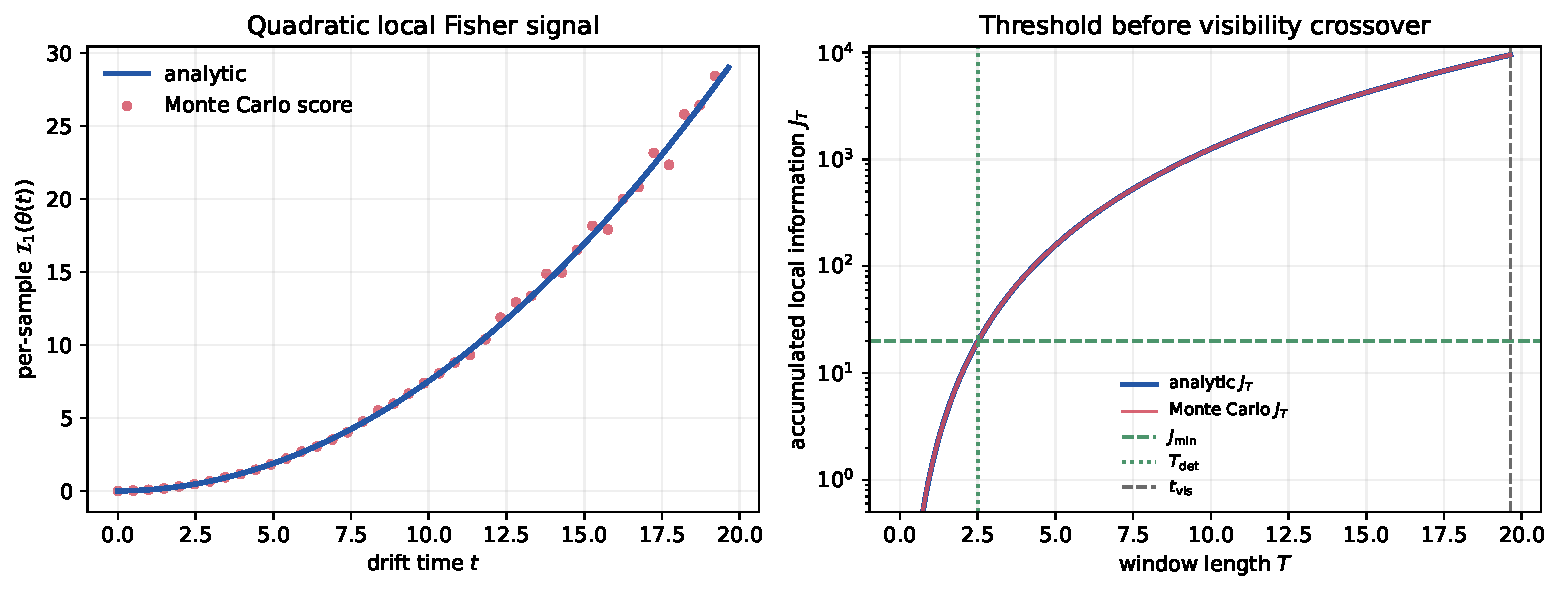
\includegraphics[width=\textwidth]{fig_fisher_residual.pdf}
\caption{\textbf{Direct score-based Fisher test.}
\textbf{Left:} analytic per-sample Fisher information and Monte Carlo
score-squared estimate, both quadratic in drift time.
\textbf{Right:} analytic and empirical accumulated local information;
the $J_{\min}=20$ crossing precedes the independently defined visibility
crossover for this parameter set.}
\label{fig:fisher_residual}
\end{figure}

% ------------------------------------------------------------
\subsection{Heuristic Calibration-Control Model}
\label{subsec:demo_model}

\paragraph{Environment.}
A $d$-dimensional linear prediction task:
$y(t) = \mathbf{w}(t)^\top \mathbf{x}(t)
+ \sigma\,\epsilon(t)$,
$\mathbf{x}(t) \sim \mathcal{N}(\mathbf{0}, \mathbf{I}_d)$,
$\epsilon \sim \mathcal{N}(0,1)$.
The weight vector $\mathbf{w}(t) \in \mathbb{S}^{d-1}$
drifts by receiving random perturbations on
\emph{background} dimensions only (indices $k,\ldots,d{-}1$),
then renormalising.  Signal therefore migrates progressively
from the ego's foreground to its blind sector.

\paragraph{Agents.}
\begin{itemize}
\item \textbf{Fixed ego} (Paper~II analogue):
  learns a linear model on a \emph{fixed} foreground
  subspace of dimension~$k$ via stochastic gradient descent
  (SGD, rate~$\eta$, decay~$\lambda$).
  Embodies the ``frozen gauge'' of Paper~II.
\item \textbf{Calibrated loop} (Paper~III analogue):
  identical ego plus a staleness sentinel and recalibration
  mechanism.
  The sentinel tracks $g_i = \mathrm{EMA}(|e\,x_i|)$ for
  each dimension~$i$ (an absolute-gradient proxy),
  computes the fraction of top-$k$ gradient dimensions
  \emph{not} in the current foreground as a frame-staleness
  index $m \in [0,1]$, and triggers
  recalibration when
  $\mathrm{EMA}(m) > \theta$.
  After recalibration, a settling period
  of~$\tau$ steps elapses before the sentinel resumes
  monitoring.
\end{itemize}

\paragraph{Parameters.}
\begin{center}
\small
\begin{tabular}{@{}lcl@{}}
\toprule
\textbf{Quantity} & \textbf{Value} & \textbf{Role} \\
\midrule
$d$ & 20 & full ambient dimension \\
$k$ & 5  & ego foreground dimension ($k/d = 0.25$) \\
$\sigma$ & 0.1 & observation noise std \\
$\eta$ & 0.01 & SGD learning rate \\
$\lambda$ & 0.998 & SGD weight decay \\
$\theta$ & 0.25 & staleness threshold \\
$\Lambda_{\mathrm{demo}}$ & variable & simulator drift amplitude per step \\
$\tau$ & variable & settling period (cooldown) \\
\bottomrule
\end{tabular}
\end{center}

\paragraph{Oracle metrics.}
Neither agent has access to $\mathbf{w}(t)$.
We evaluate performance externally using the \emph{oracle
full-space error}:
\begin{equation}
\label{eq:oracle_error}
\mathcal{E}_{\mathrm{full}}
= \bigl\|\mathbf{w}_{\mathrm{ego}}
  - \mathbf{w}^*_{\mathrm{fg}}\bigr\|^2
+ \bigl\|\mathbf{w}^*_{\mathrm{bg}}\bigr\|^2,
\end{equation}
where $\mathbf{w}^*_{\mathrm{fg}}$ and
$\mathbf{w}^*_{\mathrm{bg}}$ denote the true weight vector
restricted to foreground and background coordinates
respectively, and $\mathbf{w}_{\mathrm{ego}}$ is the ego's
foreground-supported estimator lifted to the full space.
The first term captures foreground tracking error (accessible
to the ego); the second captures hidden-sector signal
(invisible).

% ------------------------------------------------------------
\subsection{Results}
\label{subsec:demo_results}

\paragraph{Result 1: Delusion-correction separation
(Figure~\ref{fig:demo_trap}).}
At simulator drift amplitude $\Lambda_{\mathrm{demo}} = 0.02$,
settling period $\tau = 200$,
and $T = 5\,000$ steps, three phenomena are visible:

\begin{enumerate}
\item[(a)]
\emph{Delusion trap.}
The ego's foreground tracking error converges
to near zero, while the true full-space error rises
toward $\sim\!1$ and stabilises.
The growing gap between the two is the hidden sector in this supplied
linear model.  It does not prove a no-go theorem for all first-order
controllers.

\item[(b)]
\emph{Detectability.}
The staleness sentinel produces a clean sawtooth:
rising from zero after each recalibration, crossing the
threshold $\theta = 0.25$, and triggering frame reset
(25~events over $T = 5\,000$).
This demonstrates that the chosen overlap proxy can trigger a useful
reset.  The sentinel is not Fisher information; the direct Fisher test
is reported in Section~\ref{subsec:fisher_demo}.

\item[(c)]
\emph{Net benefit.}
The calibrated loop achieves
$\mathcal{E}_{\mathrm{full}} \approx 0.74$
versus the fixed ego's $\approx 1.02$:
a $27\%$ reduction in true prediction error.
\end{enumerate}

\begin{figure}[t]
\centering
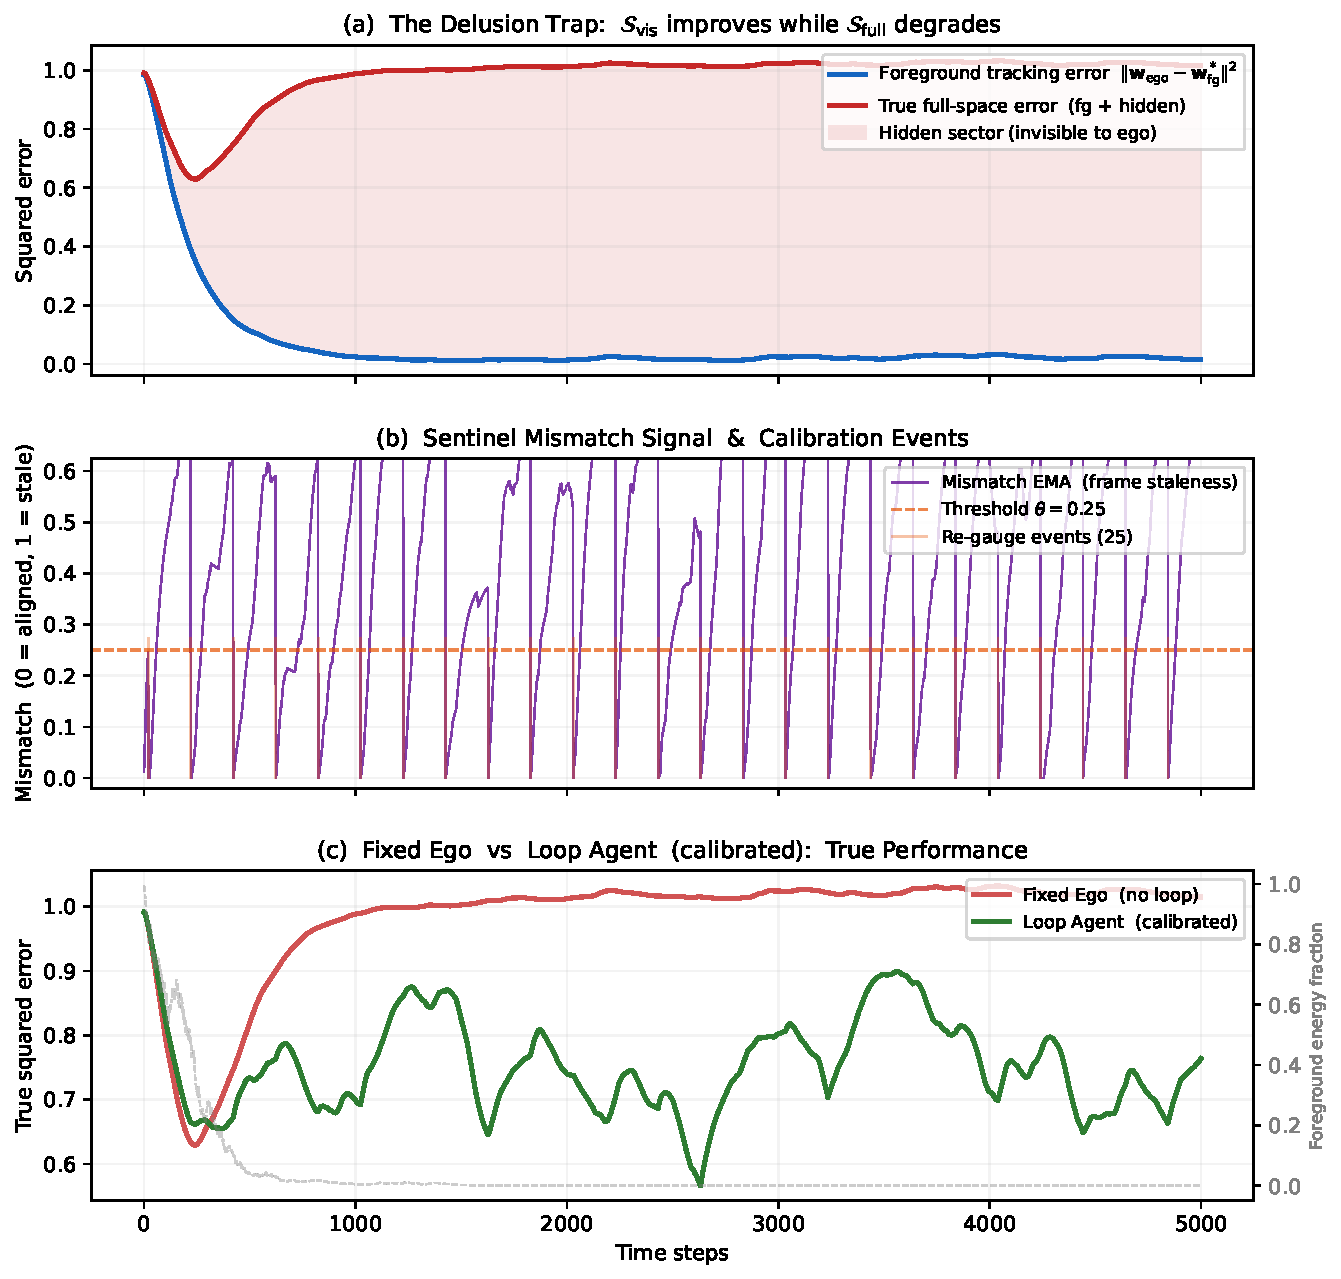
\includegraphics[width=\textwidth]{fig_delusion_trap.pdf}
\caption{%
\textbf{Delusion trap and calibration loop.}
$d = 20$, $k = 5$, $\Lambda_{\mathrm{demo}} = 0.02$,
$\tau = 200$,
$T = 5\,000$.
\textbf{(a)}~Foreground tracking error (blue) decreases
toward zero while true full-space error (red) increases;
the shaded region is the hidden sector, invisible to the ego.
\textbf{(b)}~Frame-staleness sentinel (purple) rises
monotonically between recalibration events (orange),
producing a sawtooth with 25 threshold crossings.
\textbf{(c)}~The calibrated loop (green) maintains
lower true error than the fixed ego (red);
the grey dashed line shows the foreground energy fraction
decaying as signal migrates to the background.}
\label{fig:demo_trap}
\end{figure}

\paragraph{Result 2: Phase structure and optimal
calibration budget
(Figures~\ref{fig:demo_phase}--\ref{fig:demo_alpha}).}
We scan 16 simulator drift amplitudes
$\Lambda_{\mathrm{demo}} \in [0.005, 0.08]$ and
16 settling periods $\tau \in [15, 800]$
(logarithmically spaced), running both agents for
$T = 4\,000$ steps across 6 random seeds per grid point.

Figure~\ref{fig:demo_phase}(a) shows the performance
gain $\Delta = \mathcal{E}_{\mathrm{ego}}
- \mathcal{E}_{\mathrm{loop}}$:
the loop improves over the ego (green) across most of
the parameter space, with a boundary at $\Delta = 0$
(dashed) below which recalibration is counterproductive
(very low drift, where the overhead of re-learning
exceeds the benefit of tracking).
The solid curve traces the \emph{optimal settling period}
$\tau_{\mathrm{opt}}(\Lambda_{\mathrm{demo}})$---the recalibration
period minimising $\mathcal{E}_{\mathrm{loop}}$---which
decreases monotonically from $\sim\!370$ steps at
$\Lambda_{\mathrm{demo}} = 0.005$ to $\sim\!100$ at
$\Lambda_{\mathrm{demo}} = 0.08$.
Figure~\ref{fig:demo_phase}(b) shows that calibration
frequency increases smoothly with drift and with shorter
settling period, exhibiting the cost--performance
trade-off of this supplied controller and cost proxy.  It does not test
Proposition~\ref{prop:loop_cost_impl}.

Extracting $\tau_{\mathrm{opt}}(\Lambda_{\mathrm{demo}})$ yields the
\emph{optimal calibration frequency}
$\alpha_{\mathrm{opt}}(\Lambda_{\mathrm{demo}})
= 1/\tau_{\mathrm{opt}}$
(Figure~\ref{fig:demo_alpha}).
The curve is smooth and monotonically increasing:
faster drift demands tighter calibration.
It saturates at high $\Lambda_{\mathrm{demo}}$ near
$\alpha_{\mathrm{opt}} \approx 0.01$ per step
($\tau_{\mathrm{opt}} \approx 100$), of the same
order as the learner's settling time.
This is consistent with the intuition that drift
estimation requires a minimum observation window;
the self-referential Cram\'{e}r--Rao bound
(Theorem~\ref{thm:SRCR}) provides the analytic
counterpart of this computational floor.

\begin{figure}[t]
\centering
\includegraphics[width=\textwidth]%
  {fig_phase_with_boundary.pdf}
\caption{%
\textbf{Phase structure and calibration cost.}
$16 \times 16$ grid, $T = 4\,000$, 6 seeds per point.
\textbf{(a)}~Performance gain $\Delta$; green = loop
improves on ego, red = counterproductive.
Solid curve: $\tau_{\mathrm{opt}}(\Lambda_{\mathrm{demo}})$.
Dashed: $\Delta = 0$ boundary.
\textbf{(b)}~Calibration frequency (thermodynamic cost
proxy: recalibration events per step, proportional to
energy expenditure under a fixed per-recalibration cost
model); $\tau_{\mathrm{opt}}$ overlaid.}
\label{fig:demo_phase}
\end{figure}

\begin{figure}[t]
\centering
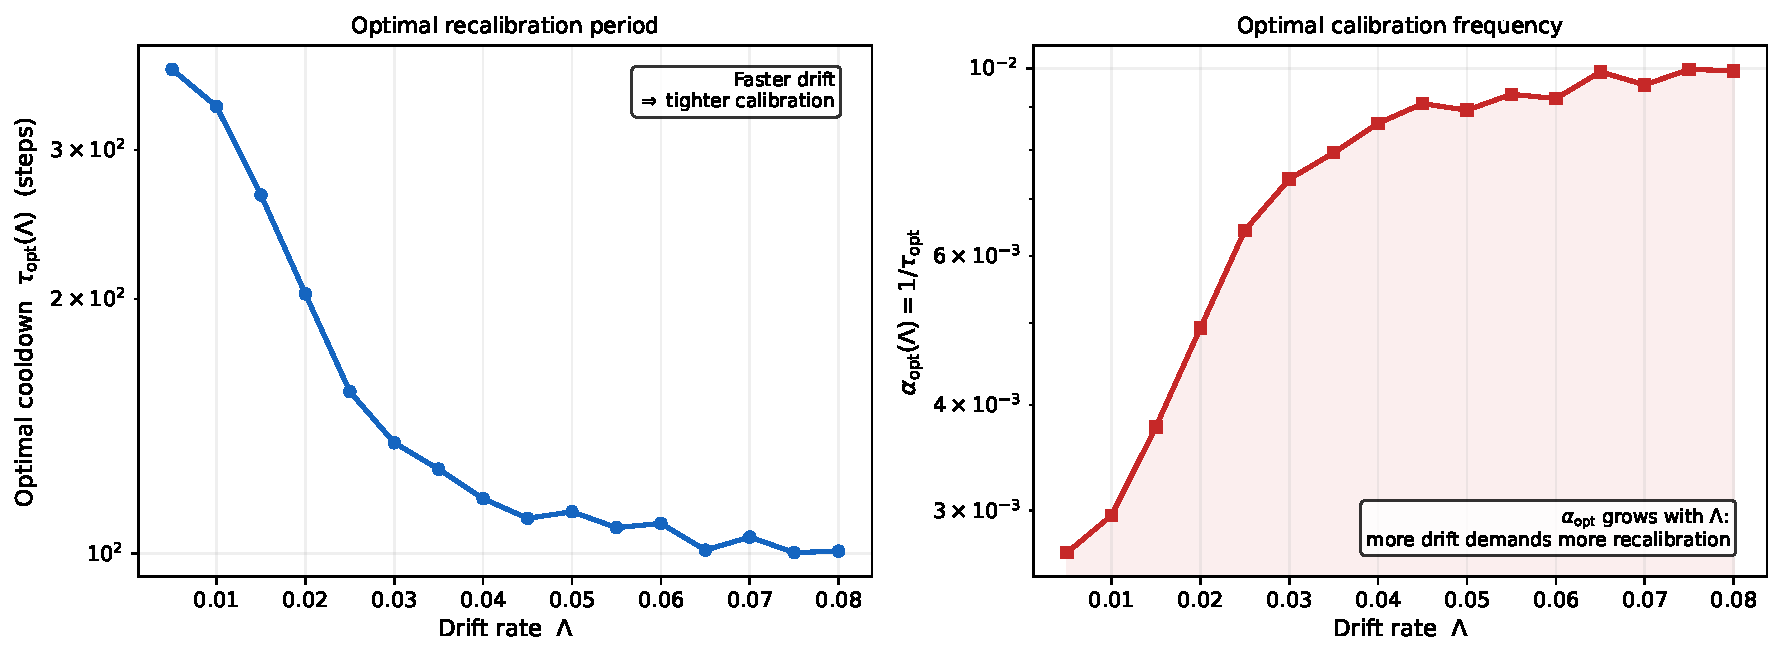
\includegraphics[width=\textwidth]{fig_alpha_opt.pdf}
\caption{%
\textbf{Optimal calibration frequency.}
\textbf{Left:}
$\tau_{\mathrm{opt}}(\Lambda_{\mathrm{demo}})$ decreases monotonically
with drift rate.
\textbf{Right:}
$\alpha_{\mathrm{opt}}(\Lambda_{\mathrm{demo}})
= 1/\tau_{\mathrm{opt}}$
increases with drift rate and saturates at the learner's
settling timescale ($\sim\!100$ steps), consistent with
an observation-window floor.}
\label{fig:demo_alpha}
\end{figure}

% ------------------------------------------------------------
\subsection{Scope of This Demonstration}
\label{subsec:demo_scope}

This demonstration \textbf{does} show:
\begin{enumerate}
\item The explicit Gaussian residual model has a directly measured
  score-squared Fisher signal with the quadratic and cubic scalings in
  Proposition~\ref{prop:gaussian_fisher}.
\item For the declared Gaussian parameters, the Fisher threshold is
  crossed before the linear visibility crossover.
\item A separate, non-Fisher frame-staleness proxy has clean threshold
  dynamics and triggers effective recalibration in the supplied linear
  controller.
\item An optimal calibration frequency
  $\alpha_{\mathrm{opt}}(\Lambda_{\mathrm{demo}})$ exists, increases
  monotonically with drift rate, and saturates at the
  learner's settling timescale in the scanned grid.
\end{enumerate}

\noindent
In summary, the direct experiment validates the declared Fisher
likelihood, while the controller experiment establishes a model-specific
proxy trade-off.  Neither is universal across architectures or
environment classes.

\medskip
This demonstration does \textbf{not} show:
\begin{enumerate}
\item That the specific functional form of
  $\alpha_{\mathrm{opt}}(\Lambda)$ matches the analytic
  Cram\'{e}r--Rao prediction in the
  large-$d$ limit.  The demonstration confirms the
  monotonic trend and saturation; deriving the exact
  scaling exponent from Theorem~\ref{thm:SRCR}
  remains open.
\item That the results generalise to all environment
  classes.  The model uses Gaussian features, linear
  regression, and isotropic background drift; extensions
  to non-linear, non-Gaussian, or structured-drift
  settings require further investigation.
\item That the calibration loop is optimal among all
  possible adaptive strategies.  It implements one
  specific realisation of the calibration-loop
  architecture.
\item That the gradient-overlap sentinel estimates Fisher information,
  or that recalibration-event frequency is a thermodynamic dissipation
  measurement.
\end{enumerate}

\paragraph{Reproducibility.}
\begin{sloppypar}
The controller simulation is in \texttt{tdome\_demo.py}.  The direct
Fisher experiment is in \texttt{fisher\_residual\_demo.py}, with raw
output in \texttt{fisher\_residual\_data.csv}.  Both require only NumPy
and Matplotlib and use fixed random seeds.
\end{sloppypar}

% ============================================================
\section{Discussion}
\label{sec:discussion}

% ------------------------------------------------------------
\subsection{Summary of Results}
\label{subsec:summary}

\begin{center}
\small
\setlength{\tabcolsep}{4pt}%
\begin{tabular}{@{}lP{6cm}c@{}}
\toprule
\textbf{Result} & \textbf{Statement} & \textbf{Sec.} \\
\midrule
Even-likelihood non-identifiability
  & The Gaussian residual record cannot identify mismatch sign
  & \ref{subsec:first_order} \\[3pt]
Drift Detectability
  & Per-sample FI is quadratic and accumulated local FI is cubic in the
    Gaussian linear-drift model
  & \ref{subsec:self_ref_fisher} \\[3pt]
Self-Referential CR Bound
  & Drift estimation bounded by
    $1/(n_{\mathrm{eff}}\,\mathbb E_\pi[\mathcal I_1]
    + \mathcal{I}_{\mathrm{ego}})$ under regular prior/likelihood data
  & \ref{subsec:SRCR} \\[3pt]
Loop Tracking Bound
  & Lyapunov $V$ with tracking neighbourhood
    $V_\infty = \|\dot{\sigma}^*\|^2/(\eta m_L)^2$ under local
    geodesic strong convexity
  & \ref{subsec:lyapunov} \\[3pt]
Four-Part Structure
  & Four supplied layers define the running model architecture
  & \ref{subsec:four_part} \\[3pt]
Loop Cost
  & $\dot{W}_{\mathrm{loop}} \geq k_BT\,\ln 2\,(R_s+R_c)
    + \mathcal{L}^2/\tau_{\mathrm{recalib}}^2$
    for a separable reset-based implementation
  & \ref{subsec:cost_theorem} \\[3pt]
Persistence Budget
  & Universal inherited budget withdrawn
  & \ref{subsec:persistence} \\[3pt]
Numerical Demonstration
  & Direct Fisher test plus a separate heuristic-controller scan
  & \ref{sec:numerical} \\
\bottomrule
\end{tabular}
\end{center}

% ------------------------------------------------------------
\subsection{Conditional Interface Sequence}
\label{subsec:logic_chain}

Papers~I--III provide a conditional interface sequence:

\begin{center}
\small
\setlength{\tabcolsep}{3pt}%
\begin{tabular}{@{}lP{3.2cm}P{3.8cm}l@{}}
\toprule
\textbf{Paper} & \textbf{Crisis} & \textbf{Resolution}
  & \textbf{What is born} \\
\midrule
Paper~I
  & Restricted autonomous baseline
  & Correlation-aware accounting
  & \textbf{Conditional resource model} \\[3pt]
Paper~II
  & Raw archive exceeds a declared budget
  & Supplied coordinate projection
  & \textbf{Frame model} \\[3pt]
Paper~III
  & Linear visibility loss in a fixed frame
  & Likelihood-based detection; conditional tracking
  & \textbf{Calibration model} \\
\bottomrule
\end{tabular}
\end{center}

The arrows are motivation or model interfaces.  The tracking theorem is
local and conditional, the universal persistence budget is withdrawn,
and no termination or completeness result follows.

% ------------------------------------------------------------
\subsection{What This Paper Does and Does Not Show}
\label{subsec:claims}

This paper \textbf{does} show:
\begin{enumerate}
\item The even Gaussian residual likelihood cannot identify mismatch
  sign, while its score has the explicit Fisher scalings in
  Proposition~\ref{prop:gaussian_fisher}.
\item Detection precedes visibility loss exactly when the threshold
  condition in Corollary~\ref{cor:detection_window} holds.
\item Drift estimation precision is bounded by the
  Self-Referential Cram\'{e}r--Rao bound
  (Theorem~\ref{thm:SRCR}).
\item The calibration loop tracks the optimal frame
  within a bounded neighbourhood under a Lyapunov
  tracking bound
  (Theorem~\ref{thm:loop_stability}).
\item A separable reset-based hardware model obeys the conditional cost
  bound in Proposition~\ref{prop:loop_cost_impl}.
\end{enumerate}

\medskip
This paper does \textbf{not} show:
\begin{enumerate}
\item That self-referential calibration implies or requires
  phenomenal consciousness, subjective experience, or
  qualia. ``Reflexivity'' as used here denotes
  second-order control, nothing more.
\item That the Lyapunov function $V$ is a measure of
  ``awareness.'' It is a control-theoretic stability
  condition, not a consciousness metric.
\item That the four-part template is necessary, sufficient, or a
  complete characterisation of agency.
\item That Fisher information requires the agent to
  ``know'' it is computing Fisher information.
  The computation can be implemented implicitly by any
  physical system whose dynamics approximate the natural
  gradient.
\item That the calibration loop eliminates the ego's bias.
  It tracks and compensates for drift in the bias;
  the four bias terms of Paper~II persist.
\item That sensing or computing is intrinsically dissipative.  The
  Landauer terms require irreversible register reset.
\item That this framework applies to all possible systems.
  It applies to systems satisfying~(C1)--(C5).
\item That the structural parallel with philosophical
  concepts of self-awareness constitutes a philosophical
  or metaphysical claim.
\item That the Clifford algebra is the only possible
  algebraic setting. Other control algebras may yield
  analogous results with different quantitative bounds.
\end{enumerate}

\medskip
We have established a checkable Gaussian Fisher signal, a regular
Bayesian estimation bound, and a local tracking result.  Their use in a
physical agent remains conditional on the declared observation,
optimization, and hardware models.

% ============================================================
% REFERENCES
% ============================================================
\begin{thebibliography}{99}

\bibitem{Liu2026TDOME_I}
S.~Liu, \emph{Non-Markovian Memory and Temporal Accumulation: A Conditional Thermodynamic Analysis}, Zenodo (2026), DOI: 10.5281/zenodo.18574342.

\bibitem{Liu2026TDOME_II}
S.~Liu, \emph{Spontaneous Symmetry Breaking of Reference Frames as a Computational Cost Minimization Strategy}, Zenodo (2026), DOI: 10.5281/zenodo.18579703.

\bibitem{Rao1945}
C.~R.~Rao,
\emph{Information and the accuracy attainable in the
estimation of statistical parameters},
Bull.\ Calcutta Math.\ Soc.\ \textbf{37}, 81 (1945).

\bibitem{Amari1985}
S.-i.~Amari,
\emph{Differential-Geometrical Methods in Statistics},
Lecture Notes in Statistics \textbf{28}, Springer (1985).

\bibitem{AmariNagaoka2000}
S.-i.~Amari and H.~Nagaoka,
\emph{Methods of Information Geometry},
Translations of Mathematical Monographs \textbf{191},
AMS (2000).

\bibitem{Amari1998}
S.-i.~Amari,
\emph{Natural gradient works efficiently in learning},
Neural Computation \textbf{10}, 251 (1998).

\bibitem{Cencov1982}
N.~N.~\v{C}encov,
\emph{Statistical Decision Rules and Optimal Inference},
Translations of Mathematical Monographs \textbf{53},
AMS (1982).

\bibitem{Crooks2007}
G.~E.~Crooks,
\emph{Measuring thermodynamic length},
Phys.\ Rev.\ Lett.\ \textbf{99}, 100602 (2007).

\bibitem{SivakCrooks2012}
D.~A.~Sivak and G.~E.~Crooks,
\emph{Thermodynamic metrics and optimal paths},
Phys.\ Rev.\ Lett.\ \textbf{108}, 190602 (2012).

\bibitem{vanTrees1968}
H.~L.~van Trees,
\emph{Detection, Estimation, and Modulation Theory},
Part~I, Wiley (1968).

\bibitem{BaratoSeifert2015}
A.~C.~Barato and U.~Seifert,
\emph{Thermodynamic uncertainty relation for biomolecular
processes},
Phys.\ Rev.\ Lett.\ \textbf{114}, 158101 (2015).

\bibitem{Ito2018}
S.~Ito,
\emph{Stochastic thermodynamic interpretation of
information geometry},
Phys.\ Rev.\ Lett.\ \textbf{121}, 030605 (2018).

\bibitem{Ashby1956}
W.~R.~Ashby,
\emph{An Introduction to Cybernetics},
Chapman \& Hall (1956).

\bibitem{vonFoerster2003}
H.~von Foerster,
\emph{Understanding Understanding: Essays on Cybernetics
and Cognition},
Springer (2003).

\bibitem{AstromWittenmark1995}
K.~J.~\AA{}str\"{o}m and B.~Wittenmark,
\emph{Adaptive Control},
2nd ed., Addison-Wesley (1995).

\bibitem{CoverThomas2006}
T.~M.~Cover and J.~A.~Thomas,
\emph{Elements of Information Theory},
2nd ed., Wiley (2006).

\bibitem{Liu2026HAFF_A}
S.~Liu, \emph{Emergent Geometry from Coarse-Grained Observable Algebras: The Holographic Alaya-Field Framework}, Zenodo (2026), DOI: 10.5281/zenodo.18361706.

\bibitem{Liu2026HAFF_B}
S.~Liu, \emph{Accessibility, Stability, and Emergent Geometry: Conceptual Clarifications on the Holographic Alaya-Field Framework}, Zenodo (2026), DOI: 10.5281/zenodo.18367060.

\bibitem{Liu2026HAFF_G}
S.~Liu, \emph{Structural Limits of Unification: Accessibility, Incompleteness, and a Programme-Level Final-Cut Diagnosis}, Zenodo (2026), DOI: 10.5281/zenodo.18402907.

\bibitem{Liu2026QRAIF_A}
S.~Liu, \emph{A Clifford-Encoding Model for Lorentzian Metrics in Entropic Gravity Frameworks}, Zenodo (2026), DOI: 10.5281/zenodo.18525876.

\bibitem{Liu2026QRAIF_B}
S.~Liu, \emph{Thermodynamic Stability Constraints on the Operator Algebra of Persistent Open Quantum Subsystems}, Zenodo (2026), DOI: 10.5281/zenodo.18525890.

\bibitem{Liu2026QRAIF_C}
S.~Liu, \emph{Conditional Image-Level Closure in the Q-RAIF Framework}, Zenodo (2026), DOI: 10.5281/zenodo.18528934.

\end{thebibliography}

\end{document}
